\item A chain $AB$ of length $l$ is located in a smooth horizontal tube so that its fraction of length $h$ hangs freely and touches the surface of the table with its end $B$ (Fig. 1.47). At a certain moment the end $A$ of the chain is set free. With what velocity will this end of the chain slip out of the tube?
    \begin{center}
        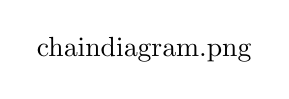
\begin{tikzpicture}
            \node at (0, 0) {{chaindiagram.png}};
        \end{tikzpicture}
    \end{center}\begin{solution}
    \begin{center}
        \begin{tikzpicture}
            \pic at (0, 0) {frame=3cm};
        \end{tikzpicture}
    \end{center}
    
    \begin{align*}
        \intertext{Let the length of the chain inside the smooth horizontal tube at an arbitrary instant be \( x \). From the equation,}
        mw &= F + u \dfrac{dm}{dt}\\
        \intertext{as \( u = 0, \mathbf{F} \uparrow \uparrow \mathbf{w} \), for the chain inside the tube}
        \lambda xw &= T, \quad \text{where} \ \lambda = \dfrac{m}{l} \tag{1}\\
        \intertext{Similarly for the overhanging part,}
        \mathbf{u} &= 0\\
        mw &= F\\
        \intertext{or}
        \lambda bw &= \lambda bg - T \tag{2}\\
        \intertext{From Eqs. (1) and (2)}
        \lambda (x + b) w &= \lambda bg\\
        \intertext{or}
        (x + b) v \dfrac{dv}{ds} &= bg\\
        \intertext{or}
        (x + b) v \dfrac{dv}{(-dx)} &= gb\\
        \intertext{(As the length of the chain inside the tube decreases with time, \( ds = -dx \).)}
        \intertext{or}
        vdv &= -gb \dfrac{dx}{x + b}\\
        \intertext{Integrating,}
        \int_{0}^{v} vdv &= -gb \int_{(l - b)}^{0} \dfrac{dx}{x + b}\\
        \intertext{or}
        \dfrac{v^2}{2} &= gb \ln \left( \dfrac{l}{b} \right)\\
        \intertext{or}
        v &= \sqrt{2gb \ln \left( \dfrac{l}{b} \right)}
    \end{align*}
\end{solution}